\begin{enumerate}[label=\thesubsection.\arabic*.,ref=\thesubsection.\theenumi]
\numberwithin{equation}{enumi}

\item
A dc amplifier has an open loop gain of 1000 and two poles, a dominant one at 1kHz and a high frequency one whose location can be controlled. It is required to connect this amplifier in a negative feedback loop that provides a dc closed loop gain of 10 and a maximally flat response.Find the required value of H.
\\
\solution Given, open loop gain G is dependent on frequency and has two poles.Therefore,G(s) can be written as..,
\begin{align}
  G(s) &= \frac{G_0}{(1+\frac{s}{p_{1}})(1+\frac{s}{p_{2}})} \label{eq:open_loop_gain} 
\end{align}
where,-p1 and -p2 are poles of G(s).
Parameters given are shown in Table.\ref{table: Input_Table}:1
\begin{table}[!ht]
\centering
\input{./tables/ee18btech11005/ee18btech11005_1.tex}
\caption{1}
\label{table: Input_Table}
\end{table}
\begin{align}
    G_0 &= 1000\\
\text{Therefore.,} G(s)&= \frac{1000}{(1+\frac{s}{p_{1}})(1+\frac{s}{p_{2}})}  
\end{align}
Let, -p1 be the dominant pole.
\begin{align}
    p_1 &= 2\pi10^3 rad/sec
\end{align}
Now, we connect the system in a negative feedback of feedback factor H.
We know that the closed loop gain of a negative feedback system is.,
\begin{align}
    T(s) &= \frac{G(s)}{1+G(s)H} \label{eq:transfer_function}
\end{align}
But,also given DC closed loop gain is 10. DC closed loop gain is given in equation.\ref{eq:dc_gain} 
\begin{align}
T(0) &= \frac{G_0}{1+G_0H} \label{eq:dc_gain} \\
\text{given.,}T(0)&=10\\
\text{and.,}G_0 &= 1000\\
\frac{1000}{1+1000H} &= 10\\
1+1000H &= 100\\
\implies H &= \frac{99}{1000} = 0.099 \label{eq:h_value}
\end{align}
from equation:\ref{eq:h_value}, the value of H is 0.099.Therefore, the feedback factor is 0.099.
%------------------------------
\item Find the location at which second ple can be placed.\\
\solution Given the negative feedback system should have maximally flat response.from equation.\ref{eq:transfer_function} and equation.\ref{eq:open_loop_gain} the transfer function is,
\begin{align}
    T(s) &= \frac{\frac{G_0}{(1+\frac{s}{p_{1}})(1+\frac{s}{p_{2}})}}{1+\frac{HG_0}{(1+\frac{s}{p_{1}})(1+\frac{s}{p_{2}})}}\\
    T(s) &= \frac{\frac{p_1p_2G_0}{(p_1+s)(p_2+s)}}{1+\frac{p_1p_2HG_0}{(p_1+s)(p_2+s)}}
\end{align}
\begin{align}
    T(s) &= \frac{p_1p_2G_0}{(p_1+s)(p_2+s) + p_1p_2HG_0}\\
    T(s) &= \frac{p_1p_2G_0}{p_1p_2+(p_1+p_2)s+s^2 + p_1p_2HG_0}\\
    T(s) &= \frac{p_1p_2G_0}{s^2+(p_1+p_2)s+(HG_0+1)p_1p_2} \label{eq:closed_loop}
\end{align}
The characteristics equation of above transfer function is.,
\begin{align}
    C.E &= s^2+(p_1+p_2)s+(HG_0+1)p_1p_2 \label{eq:ce}
\end{align}
In general, For a second order amplifier the C.E is.,
\begin{align}
    C.E &= s^2+2\zeta\omega_ns+\omega_n^{2} \label{eq:second_order_ce}
\end{align}
The quality factor Q of equation.\ref{eq:second_order_ce}, is given by
\begin{align}
    Q &= \frac{1}{2\zeta}
\end{align}
From equation.\ref{eq:ce},
\begin{align}
    \omega_n &= \pm{\sqrt{(HG_0+1)p_1p_2}}\\
    \zeta &= \pm{\frac{2p_1p_2}{\sqrt{(HG_0+1)p_1p_2}}}
\end{align}
Therefore,For the given second order amplifier with characteristic equation.\ref{eq:ce},the Q factor is,
\begin{align}
    Q &= \pm{\frac{\sqrt{(1+HG_0)p_1p_2}}{p_1+p_2}} \label{eq:Q}
\end{align}
For a negative feedback amplifier to achieve maximally flat response,
\begin{align}
    Q &= 0.7071\\
\end{align}
Therefore, substituting the values of Q and other parameters in equation.\ref{eq:Q},
\begin{align}
    0.7071 &= \pm{\frac{\sqrt{(1+0.099(1000))(2\pi10^3)p_2}}{2\pi10^3+p_2}}
\end{align}
Squaring on both sides and rearranging.,
\begin{align}
    (1+1000(0.099))2\pi10^3p_2 &= 0.7071^2{(2\pi10^3+p_2)}^2
\end{align}
\begin{align}
    (100)2\pi10^3 = 0.7071^2(2\pi10^3+p_2)^2\\
    \implies 0.5p_2^2-622037.2p_2+19733247.6=0
\end{align}
Solving above equation.,
\begin{align}
p_2 &= 31.7244 \text{ rad/sec}\\
p_2 &= 1244042.676 \text{ rad/sec}
\end{align}
But, Since p1 is dominating pole,p1 should be close to origin.
\begin{align}
    p_1 <<< p_2
\end{align}
\begin{align}
p_2 &= 1.244\text{ Mrad/sec}\\
\\
p_2 &= \frac{1.244M}{2\pi} \text{Hz}\\
&= 197.989\text{ kHz}\\
\end{align}
\textbf{The second pole frequency is 1.244 Mrad/sec}
\textbf{NOTE:-} The poles are at -p1 and -p2,where p1 and p2 are positive numbers.Therefore poles lie on left half of s-plane.So the system is stable.
%---------------------
\item Verify roots of above equation using python code.
\begin{lstlisting}
codes/ee18btech11005/ee18btech11005_1.py
\end{lstlisting}
%-----------------
\item Find the open loop transfer function and closed loop transfer function of the system.
\solution Substituting the value of p2 in  the equation \ref{eq:open_loop_gain} and \ref{eq:closed_loop}
\begin{align}
     G(s) &= \frac{1000}{(1+\frac{s}{2\pi10^3})(1+\frac{s}{1.244x10^6})}
\end{align}
\begin{align}
    T(s) &= \frac{7.816x10^{12}}{s^2+125x10^4s+7.816x10^{11}} \\
    T(s) &= \frac{10}{0.128x10^{-11}s^2+1.599x10^{-6}s+1}
    \label{eq:Transfer_func}
\end{align}
%--------------------------
\item Verify from the Bode plot of above closed loop transfer function that it has maximally flat response.\\
\solution The following code generates the bode plot of the transfer function.
\begin{lstlisting}
codes/ee18btech11005/ee18btech11005_2.py
\end{lstlisting}
\begin{figure}[!ht]
\centering
\includegraphics[width=\columnwidth]{./figs/ee18btech11005/ee18btech11005_1.eps}
\caption{1}
\label{fig:ee18btech11005_1}
\end{figure}
From the magnitude bode plot in figure.\ref{fig:ee18btech11005_1}:1 we can tell that the open loop transfer function after having negative feedback has maximally flat response for the obtained value of p2. 
%---------------------------------
\item Find the step response of above closed loop system.\\
\solution The following code generates the unit step response of closed loop transfer function.
\begin{lstlisting}
codes/ee18btech11005/ee18btech11005_3.py
\end{lstlisting}
The plot of unit step response is shown in the figure.\ref{fig:ee18btech11005_2}
\begin{figure}[!ht]
\centering
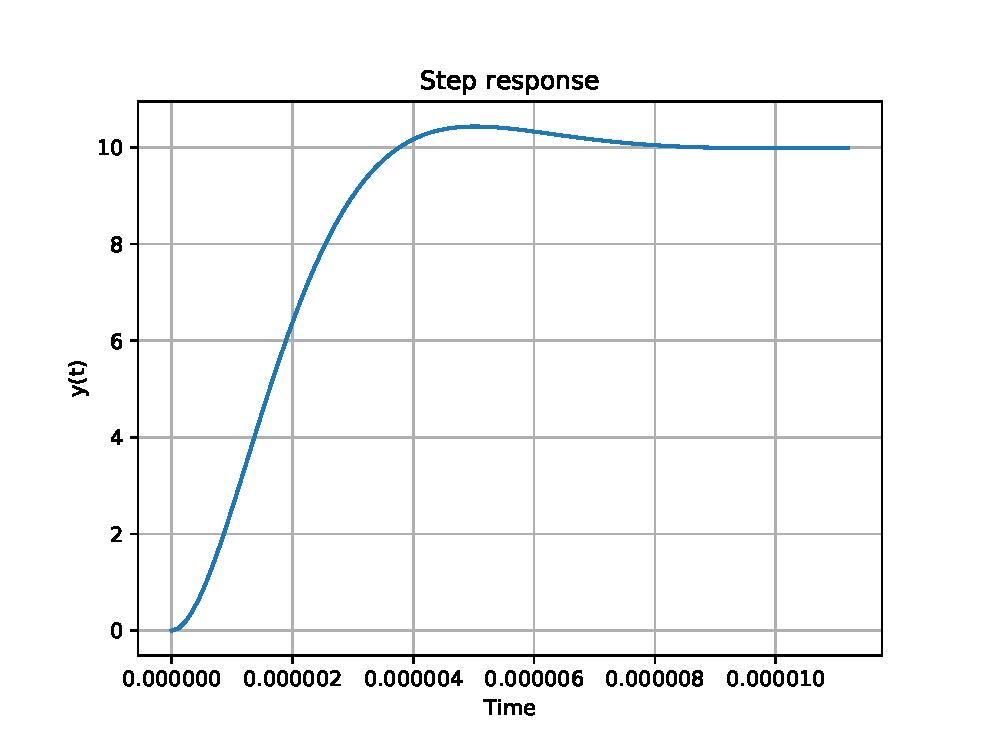
\includegraphics[width=\columnwidth]{./figs/ee18btech11005/ee18btech11005_2.eps}
\caption{}
\label{fig:ee18btech11005_2}
\end{figure}

%-------------------------------
\item Design a circuit that represents the above transfer function.\\
\solution The circuit can be designed using an operational amplifiers having negative feedback.Consider the circuit shown in figure.\ref{fig:equivalent_control_system}:1.Assume the gain of all the amplifiers are large.And assume no zero state response.Take the parameters in s-domain.\\
\begin{figure}[!hbt]
	\begin{center}
			\resizebox{\columnwidth}{!}{
 \begin{circuitikz}
\ctikzset{bipoles/length=1cm}

\draw 
(0, 0) node[op amp] (opamp) {}
(4.5, -0.35) node[op amp] (opamp2) {}
(9, -0.7) node[op amp] (opamp3) {}
(13,-1.05) node[op amp] (opamp4) {}
(opamp.-) -- (-1,0.35) -- (-1.5,0.35) to[R=$R_1$] (-3,0.35){}
(-1,0.35)-- (-1,1) to[R=$R_2$] (1.5,1) -- (1.5,0){}
(1.5,0)--(2,0) to[R=$R$] (3,0)--(3.5,0)--(opamp2.-){}
(opamp2.+)--(3.5,-0.7) node[ground]{}
(opamp.out)--(1.5,0){}
(opamp.+) -- (-1,-0.35) node[ground]{}
(3.5,0) -- (3.5,0.75)--(4,0.75) to[R=$R$] (6,0.75) -- (6,-0.35){}
(3.5,0.75)--(3.5,1.5) to[C=$C$] (6,1.5)--(6,0.35){}
(opamp2.out) -- (6,-0.35){}
(6,-0.35)--(6.5,-0.35) to[R=$R$] (7.5,-0.35)--(8,-0.35)--(opamp3.-){}
(opamp3.+)--(8,-1.05) node[ground]{}
(8,-0.35) -- (8,0.75) to[R=$R$] (10,0.75) -- (10,-0.7){}
(opamp3.out) -- (10,-0.7){}
(10,-0.7)--(10.5,-0.7) to[R=$R$] (11.5,-0.7)--(12,-0.7)--(opamp4.-) {}
(12,-0.7) -- (12,0.05) to[C=$C_1$] (14,0.05) -- (14,-1.05){}
(14,-1.05) -- (15,-1.05){}
(opamp4.out) -- (14,-1.05){}
(opamp4.+)--(12,-1.4) node[ground]{}
(3.5,0.75)--(3.5,2.5) to[R=$R$] (14,2.5) -- (14,-1.05){}
node at (-1,0.2){A}
node at (3.5,-0.2){B}
node at (8,-0.7) {C}
node at (12,-1){D}

node at (1.5,-0.4){$V_1$}
node at (6,-0.6){$V_2$}
node at (10,-1){$V_3$}
node at (15,-1.4) {$V_{out}$}
node at(-3,0.7){$V_{in}$}

;\end{circuitikz}



}
	\end{center}
\caption{1}
\label{fig:equivalent_control_system}
\end{figure}
\textbf{For the first amplifier..,}
Applying KCL at node A., 
Since, the opamp has large gain, potential at node A is assumed to be zero due to virtual short at node A.
\begin{align}
    \frac{0-V_{in}(s)}{R_1} +\frac{0-V_1(s)}{R_2} &= 0\\
    \frac{V_{in}(s)}{R_1} &= \frac{V_1(s)}{R_2}\\
\implies V_{in} &= -\frac{V_1(s) R_1}{R_2}\label{eq:opamp_1}
\end{align}
\textbf{For the second amplifier..,}
Applying KCL at node B..,
Similarly potential at node B is zero.
\begin{align}
  \frac{-V_1(s)}{R}+\frac{-V_2(s)}{R}-sCV_2(s)+\frac{-V_{out}(s)}{R} &= 0\\
  \frac{-V_1(s)}{R}+\frac{-V_2(s)}{R}-sCV_2(s) = \frac{V_{out}(s)}{R} \\
  \frac{-V_1(s)}{R} = V_2(s)\sbrak{sC+\frac{1}{R}}+\frac{V{out}(s)}{R} \label{eq:opamp_2}
\end{align}
\textbf{For the third amplifier..,}
Potential at node C is zero(Due to high gain of amplifier).Applying KCL at node C.
\begin{align}
    \frac{-V_2(s)}{R}+\frac{-V_3(s)}{R} = 0\\
    \implies V_2(s) = -V_3(s) \label{eq:opamp_3}
\end{align}
\textbf{For the Fourth amplifier.,}
Potential at node D is zero.Applying KCL at node D.
\begin{align}
    \frac{-V_3(s)}{R}+sC_1(-V_{out}(s)) = 0\\
    V_3(s) = -sC_1RV_{out}(s) \label{eq:opamp_4}
\end{align}
From equation.\ref{eq:opamp_4} and equation. \ref{eq:opamp_3}..,
\begin{align}
    V_2(s) = sC_1RV_{out}(s) \label{eq:eq_1}
\end{align}
Substituting the equation.\ref{eq:opamp_2} and equation.\ref{eq:eq_1},
\begin{align}
    \frac{-V_1(s)}{R} &= (s^2C_1CR + sC_1)V_{out}(s) +\frac{V_{out}(s)}{R}\\
    V_1(s) &= -(s^2C_1CR^2+sC_1R+1)V_{out}(s)\label{eq:eq_2}
\end{align}
from equation.\ref{eq:opamp_1} and equation.\ref{eq:eq_2}.
\begin{align}
     V_1(s) &= \frac{R_1}{R_2}(s^2C_1CR^2+sC_1R+1)V_{out}(s)\\
    \frac{V_{out}(s)}{V_{in}(s)} &= \frac{R_2}{R_1(s^2C_1CR^2+sC_1R+1)} \label{eq:eq_3}
\end{align}
Comparing equation.\ref{eq:Transfer_func} and equation.\ref{eq:eq_3}
\begin{align}
    \frac{R_2}{R_1} &= 10 \\
    C_1CR^2 &= 0.128x10^{-11} \\
    C_1R &= 1.599x10^{-6} F\\
\text{Let.,} R &= 1000 \Omega\\
\implies C_1 &= 1.599x10^{-9} \\
 \text{and.,} C_1CR^2 &= 0.128x10^{-11} \\
 \implies C &= 0.8005x10^{-9} F
\end{align}
\begin{align}
\text{Let..,} R_1 &= 100\Omega\\
\implies R_2 &= 1000\Omega
\end{align}
\begin{table}[!ht]
\centering
\input{./tables/ee18btech11005/ee18btech11005_2.tex}
\caption{1}
\label{table: Output_Table}
\end{table}
From Table.\ref{table: Output_Table}:1. The Final circuit is shown in figure.\ref{fig:Final_circuit}
\begin{figure}[!hbt]
	\begin{center}
			\resizebox{\columnwidth}{!}{\begin{circuitikz}
\ctikzset{bipoles/length=1cm}

\draw 
(0, 0) node[op amp] (opamp) {$1$}
(4.5, -0.35) node[op amp] (opamp2) {$2$}
(opamp.-) -- (-1,0.35) -- (-1.5,0.35) to[R=$1k\Omega$] (-3,0.35){}
(-1,0.35)-- (-1,1) to[C=$1nF$] (1.5,1) -- (1.5,0){}
(1.5,0)--(2,0) to[R=$1k\Omega$] (3,0)--(3.5,0)--(opamp2.-){}
(opamp2.+)--(3.5,-0.7) node[ground]{}
(opamp.out)--(1.5,0){}
(opamp.+) -- (-1.5,-0.35) -- (-1.5,-1.5) 
(6,-1.5) to[C=$0.599nF$] (6,-3) node[ground]{}
(-1.5,-1.5) to[R=$1k\Omega$] (6,-1.5) --(6,-0.35){}
(3.5,0) -- (3.5,0.75)--(4,0.75) to[C=$0.681nF$] (6,0.75) -- (6,-0.35){}
(opamp2.out) -- (6,-0.35){}
(6,-0.35)--(6.5,-0.35)
node at (-1,0.2){A}
node at (3.5,-0.2){B}
node at (1.5,-0.4){$V_1$}
node at (6.3,-0.6){$V_{out}$}
node at(-3,0.7){$V_{in}$}

;\end{circuitikz}

}
	\end{center}
\caption{1}
\label{fig:Final_circuit}
\end{figure}
\end{enumerate}



